\section{Scenario d'esempio}

Per meglio comprendere l'architettura di sistema appena descritta e le interazioni tra i suoi componenti costituenti, si prende a riferimento uno scenario d'esempio chiamato "recycling robots". Come si può intuire dal nome, la scena contiene dei robot, i quali hanno il compito di riciclare la spazzatura presente nell'ambiente portandola in un bidone.

\medskip

Il compito generale di un robot è divisibile in un ciclo di sotto-obiettivi, ad esempio:
\begin{enumerate}
    \item Cercare la spazzatura;
    \item Andare verso la spazzatura trovata;
    \item Prendere la spazzatura appena raggiunta;
    \item Cercare il bidone
    \item Andare verso il bidone trovato
    \item Riciclare la spazzatura
\end{enumerate}

Utilizzando il formalismo di Jason, i sotto-obiettivi elencati sono associabili a dei \textit{"plans"} di un agente. Al di fuori del primo plan (Cercare la spazzatura), normalmente attivato dal \textit{"goal"} principale presente nell'agente, i successivi possono essere attivati da una percezione ricevuta dall'agente. Ad esempio, in risposta alla ricerca del bidone è possibile notificare la scoperta di un bidone nelle vicinanze e, di conseguenza, fare in modo che l'agente utilizzi il plan "Andare verso il bidone trovato".

\begin{figure}[H]
\centering
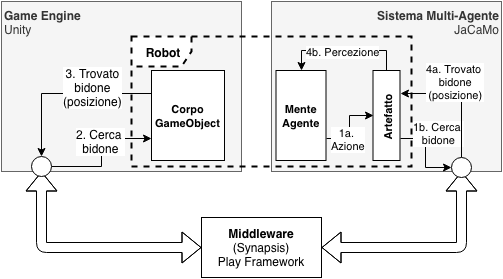
\includegraphics[width=0.7\textwidth]{figures/Esempio_relazione.png}
\caption{Esempio di comunicazione tra mente e corpo}
\end{figure}

L'immagine mostra il flusso ordinato di interazioni per l'esempio appena descritto. La mente per svolgere il plan \textit{"Cercare il bidone"} vuole inviare al proprio corpo l'azione \textit{"Cerca bidone"}. La richiesta di svolgere l'azione inizia dall'utilizzo dell'operazione presente nell'artefatto personale dell'agente\footnote{previa associazione dei due}, in possesso del canale per comunicare con il middleware.

\begin{figure}[H]
\centering
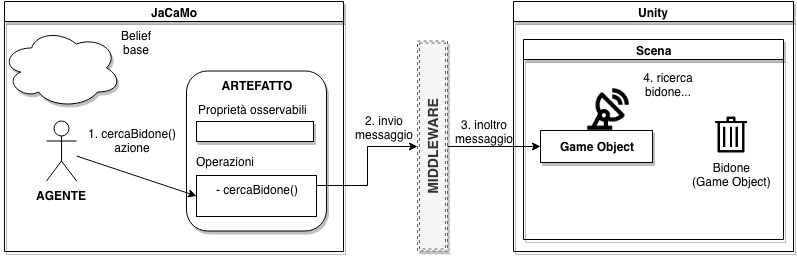
\includegraphics[width=\textwidth]{figures/da_Agente_a_Game_Object.png}
\caption{Fase in invio azione a GameObject}
\end{figure}

L'artefatto quindi invia il messaggio al middleware che si occupa di inoltrare le informazioni al Game Object. Alla ricezione delle stesse, l'entità corpo (GameObject) attua l'azione richiesta e risponde alla mente (Agente) inviandogli la percezione generata, ad esempio \textit{"trovato(nomeBidone,posizione)"}.

\begin{figure}[H]
\centering
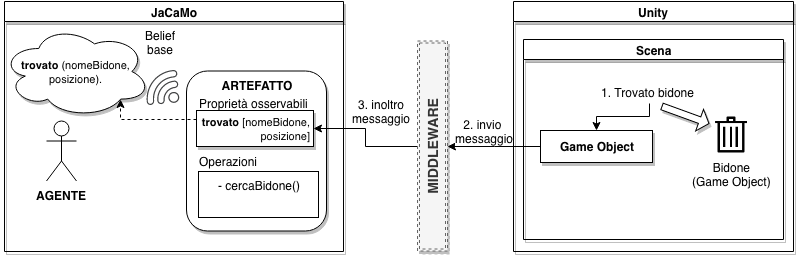
\includegraphics[width=\textwidth]{figures/da_Game_Object_a_Agente.png}
\caption{Fase di invio percezione ad Agente}
\end{figure}

A questo punto la percezione viene mandata al middleware che, a sua volta, la inoltrerà all'artefatto collegato. L'artefatto, nel momento in cui riceve la percezione, aggiunge quest'ultima alle sue proprietà osservabili che, automaticamente, aggiorneranno la BeliefBase dell'agente. L'ultimo passaggio rappresenta il punto cruciale per completare il collegamento tra corpo e mente dato che in questa maniera l'agente ha ricevuto la percezione dal proprio corpo. 

\medskip

Si intende inoltre lasciare aperta la possibilità, da parte del corpo, di inviare percezioni non come reazione ad azioni eseguite dalla mente, dato che il collegamento WebSocket, una volta effettuato, rimane attivo per tutta la durata di vita dell'entità. Ad esempio, in caso di contatto con un oggetto nella scena Unity, il corpo deve essere in grado di mandare una percezione del tipo \textit{"toccata(nome\_oggetto,posizione)"} alla propria mente senza bisogno di stimoli.
